%%
%%

\chapter{D\'emarrer avec Bacula}
\label{_ChapterStart37}
\index[general]{Bacula!D\'emarrer avec }
\index[general]{D\'emarrer avec Bacula }

Si vous \^etes comme moi, vous voulez faire fonctionner Bacula imm\'ediatement
pour en avoir un aper\c{c}u, puis, plus tard, vous reviendrez en arri\`ere
pour lire et conna{\^\i}tre tous les d\'etails. C'est exactement ce que ce
chapitre se propose d'accomplir : vous faire avancer rapidement sans tous les
d\'etails. Si vous voulez sauter la section sur les Pools, Volumes et Labels,
vous pourrez toujours y revenir, mais s'il vous pla\^it, veuillez lire ce
chapitre jusqu'\`a la fin, et en particulier suivre les instructions pour
tester votre lecteur de bandes. 

Nous supposons que vous \^etes parvenus \`a construire et installer Bacula,
sinon, vous devriez d'abord jeter un oeil aux 
\ilink{Pr\'erequis (syst\`eme)}{SysReqs} puis au chapitre 
\ilink{Compiler et installer Bacula}{_ChapterStart17} de ce manuel. 

\label{JobsandSchedules}
\section{Comprendre les Jobs et Schedules}
\index[general]{Jobs!Comprendre}
\index[general]{Schedules!Comprendre}
\addcontentsline{toc}{section}{Comprendre les Jobs et Schedules}

Afin de rendre Bacula aussi flexible que possible, les directives lui sont 
donn\'ees en plusieurs endroits. L'instruction principale est la ressource Job, 
qui d\'efinit un job. Un job de type sauvegarde consiste en g\'en\'eral en un 
FileSet, un client, un Schedule pour un ou plusieurs niveaux ou horaires de sauvegardes, 
un Pool, ainsi que des instructions additionnelles. Un autre point de vue 
est de consid\'erer le FileSet comme "Que sauvegarder ?", le Client comme 
"Qui sauvegarder ?", le Schedule comme "Quand sauvegarder ?" et le Pool 
comme "O\`u sauvegarder ?" (c'est \`a dire, "Sur quel volume ?)

Typiquement, une combinaison FileSet/Client aura un job correspondant. La plupart 
des directives, telles que les FileSets, Pools, Schedules, peuvent \^etre 
m\'elang\'ees et partag\'ees entre les jobs. Ainsi, vous pouvez avoir deux d\'efinitions 
(ressources) de jobs sauvegardant diff\'erents serveurs et utilisant les m\^emes 
Schedule, FileSet (sauvegardant donc les m\^emes r\'epertoires sur les deux 
machines) et peut-\^etre m\^eme les m\^emes Pools. Le Schedule d\'efinira quel 
type de sauvegarde sera ex\'ecut\'e et \`a quel moment (par exemple les Full le 
mercredi, les incr\'ementales le reste de la semaine), et lorsque plus d'un job 
utilise le m\^eme Schedule la priorit\'e du job d\'etermine lequel d\'emarre en premier. 
Si vous avez de nombreux jobs, vous devriez utiliser la directive JobDefs, 
qui vous permet de d\'efinir des param\`etres par d\'efaut pour vos jobs, qui peuvent \^etre 
chang\'es au sein de la ressource Job, mais qui vous \'evitent de r\'e\'ecrire les m\^emes 
param\`etres pour chaque job. En plus des FileSets que vous voulez sauvegarder, 
vous devriez aussi avoir un job qui sauvegarde votre catalogue.

Enfin, sachez qu'en plus des jobs de type Backup, vous pouvez aussi utiliser 
des jobs de type restore, verify, admin, qui ont chacun des exigences 
diff\'erentes.

\label{PoolsVolsLabels}

\section{Comprendre les Pools, Volumes et Labels}
\index[general]{Comprendre les Pools, Volumes et Labels }
\index[general]{Labels!Comprendre les Pools Volumes et }
\addcontentsline{toc}{section}{Comprendre les Pools, Volumes et Labels}

Si vous avez utilis\'e un programme tel que {\bf tar} pour sauvegarder votre
syst\`eme, les notions de Pools, Volumes et labels peuvent vous sembler un peu
confuses au premier abord. Un Volume est un simple support physique
(cartouche, ou simple fichier) sur lequel Bacula \'ecrit vos donn\'ees de
sauvegarde. Les Pools regroupent les Volumes de sorte qu'une sauvegarde n'est
pas restreinte \`a la capacit\'e d'un unique Volume. Par cons\'equent,
plut\^ot que de nommer explicitement les Volumes dans votre Job, vous
sp\'ecifiez un Pool, et Bacula se chargera de s\'electionner le prochain
Volume utilisable du Pool et vous demandera de le monter. 

Bien que les options de base soient sp\'ecifi\'ees dans la ressource Pool du
fichier de configuration du Director, le Pool {\bf r\'eel} est g\'er\'e par le
Catalogue Bacula. Il contient les informations de la ressource Pool
(bacula-dir.conf) ainsi que les informations concernant tous les Volumes qui
ont \'et\'e ajout\'es au Pool. L'ajout de Volumes se fait en principe
manuellement depuis la Console gr\^ace \`a la commande {\bf label}. 

Pour chaque Volume, Bacula g\`ere une quantit\'e d'informations consid\'erable
telles que les premi\`ere et derni\`ere date et heure d'\'ecriture, le nombre
de fichiers sur le Volume, le nombre de bytes sur le Volume, le nombre de
montages, etc. 

Pour que Bacula puisse lire ou \'ecrire sur un Volume physique, celui-ci doit
avoir re\c{c}u un \'etiquettage logiciel afin que Bacula soit assur\'e que le
bon Volume est mont\'e. Ceci s'effectue en principe manuellement depuis la
Console gr\^ace \`a la commande {\bf label}. 

Les \'etapes de cr\'eation de Pool, ajout de Volumes \`a ce Pool, et
\'ecriture d'\'etiquettes logicielles sur les Volumes, peuvent sembler
p\'enibles au premier abord, mais en fait, elles sont tout \`a fait simples
\`a franchir, et elles vous permettent d'utiliser plusieurs Volumes (plut\^ot
que d'\^etre limit\'e \`a la capacit\'e d'un seul). Les Pools vous procurent
aussi une flexibilit\'e importante pour votre politique de sauvegarde. Par
exemple, vous pouvez avoir un Pool de Volumes "Daily" pour vos sauvegardes
Incr\'ementales et un Pool de Volumes "Weekly" pour vos sauvegardes
compl\`etes (Full). En sp\'ecifiant le Pool appropri\'e dans les Jobs de
sauvegarde quotidiens et hebdomadaires, vous garantissez qu'aucun Job
quotidien n'\'ecrira jamais sur un Volume du Pool r\'eserv\'e aux sauvegardes
hebdomadaire et vice versa, et Bacula vous dira quelle cartouche est requise,
et quand. 

Pour plus de d\'etails concernant les Pools, consultez la section 
\ilink{Ressource Pool}{PoolResource} du chapitre sur la
configuration du Director, ou poursuivez votre lecture, nous reviendrons plus
tard sur ce sujet. 

\section{Param\'etrage des fichiers de configuration de Bacula}
\label{config}
\index[general]{Param\'etrage des fichiers de configuration de Bacula }
\index[general]{Bacula!Param\'etrage des fichiers de configuration de }
\addcontentsline{toc}{section}{Param\'etrage des fichiers de configuration
de Bacula}

Apr\`es avoir ex\'ecut\'e la commande {\bf ./configure} {\it ad hoc}, {\bf
make} et {\bf make install}, si c'est la premi\`ere fois que vous ex\'ecutez
Bacula, vous devez cr\'eer des fichiers de configuration valides pour le
Director, le File Daemon, le Storage Daemon et le programme Console. Si vous
avez suivi nos recommandations, des fichiers de configuration par d\'efaut
ainsi que les binaires des {\it daemons} seront situ\'es dans votre
r\'epertoire d'installation. Dans tous les cas les binaires se trouvent dans
le r\'epertoire que vous avez sp\'ecifi\'e au niveau de l'option {\bf
\verb{--{sbindir} de la commande {\bf ./configure}, et les fichiers de configuration
se trouvent dans le r\'epertoire que vous avez sp\'ecifi\'e au niveau de
l'option {\bf \verb{--{sysconfdir}. 

Lors des param\'etrages initiaux de Bacula, il vous faudra investir un peu de
temps pour modifier les fichiers de configuration par d\'efaut afin de
les adapter \`a votre environnement. Ceci peut n\'ecessiter de red\'emarrer
Bacula plusieurs fois jusqu'\`a ce que tout fonctionne correctement. Ne
c\'edez pas au d\'esespoir. Une fois que vous aurez cr\'e\'e vos fichiers de
configuration, vous n'aurez que rarement besoin de les changer et de
red\'emarrer Bacula. Le gros du travail consistera \`a changer la cartouche
quand elle est pleine. 

\subsection{
\ilink{Configurer le programme Console}{_ChapterStart36}}
\index[general]{Console!Configurer le programme }
\index[general]{Configurer le programme Console }
\addcontentsline{toc}{subsection}{Configurer le programme Console}

Le programme console est utilis\'e par l'administrateur pour interagir avec le
Director et pour arr\^eter et d\'emarrer manuellement des jobs, ou encore pour
obtenir des informations sur les jobs en cours d'ex\'ecution ou programm\'es.

Le fichier de configuration de la Console se trouve dans le r\'epertoire que
vous avez sp\'ecifi\'e au niveau de l'option {\bf \verb{--{sysconfdir} de la commande
{\bf ./configure} et par d\'efaut se nomme {\bf console.conf}.

Si vous avez choisi de construire la Console GNOME avec l'option {\bf
\verb{--{enable-gnome}, vous y trouverez \'egalement son fichier de configuration par
d\'efaut, nomm\'e {\bf gnome-console.conf}. 

Il en va de m\^eme pour la console wxWidgets, qui est construite par l'option
{\bf \verb{--{enable-bwx-console}, et le nom du fichier de configuration par d\'efaut
est, dans ce cas, {\bf bwx-console.conf}. 

Normalement, pour les nouveaux
utilisateurs, aucune modification n'est requise pour ces fichiers. Les
r\'eglages par d\'efaut sont raisonnables. 

\subsection{
\ilink{Configurer le programme Monitor}{_ChapterStart35}}
\index[general]{Monitor!Configurer le programme }
\index[general]{Configurer le programme Monitor }
\addcontentsline{toc}{subsection}{Configurer le programme Monitor}

Le programme Monitor est typiquement une ic\^one dans la barre des t\^aches.
Cependant, lorsque l'ic\^one est \'etendue en une fen\`etre, l'administrateur ou
l'utilisateur peut obtenir des informations concernant le Director ou l'\'etat
des sauvegardes sur la machine locale ou n'importe quelle autre {\it daemon}
Bacula configur\'e. 

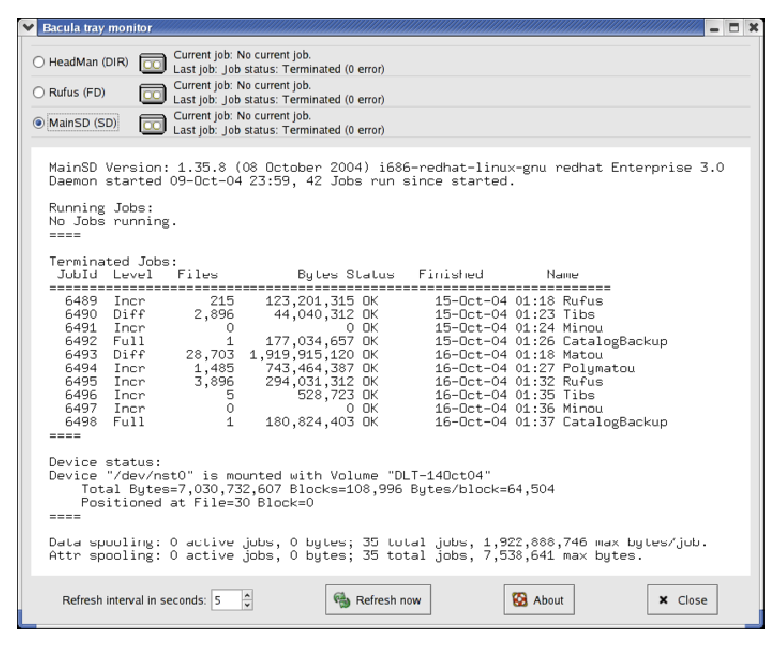
\includegraphics{./Bacula-tray-monitor.eps} 

L'image montre le tray-monitor configur\'e pour trois {\it daemons}. En
cliquant sur les boutons radio dans le coin en haut \`a gauche de l'image,
vous pouvez voir l'\'etat de chacun des {\it daemons}. L'image montre l'\'etat
du Storage Daemon (MainSD) s\'electionn\'e. 

Le fichier de configuration du Monitor se trouve dans le r\'epertoire
sp\'ecifi\'e au niveau de l'option {\bf \verb{--{sysconfdir} de la commande {\bf
./configure} et se nomme par d\'efaut {\bf tray-monitor.conf}. En principe,
pour les nouveaux utilisateurs, il suffit de changer les permissions de ce
fichier pour permettre aux utilisateurs non-root d'ex\'ecuter le Monitor, en
effet cette application doit \^etre ex\'ecut\'e par le m\^eme utilisateur que
l'environnement graphique (n'oubliez pas de donner aux non-root le droit
d'ex\'ecuter {\bf bacula-tray-monitor}). Ceci ne constitue pas une faille de
s\'ecurit\'e tant que vous utilisez les r\'eglages par d\'efaut. 

\subsection{
\ilink{Configurer le File Daemon}{_ChapterStart25}}
\index[general]{Configurer le File Daemon }
\index[general]{Daemon!Configurer le File }
\addcontentsline{toc}{subsection}{Configurer le File Daemon}

Le File Daemon, est le programme qui s'ex\'ecute sur chaque machine cliente. A
la demande du Director, il d\'etermine les fichiers \`a sauvegarder et les
exp\'edie au Storage Daemon. 

Le fichier de configuration du File Daemon se trouve dans le r\'epertoire
sp\'ecifi\'e au niveau de l'option {\bf \verb{--{sysconfdir} de la commande {\bf
./configure} et se nomme par d\'efaut {\bf bacula-fd.conf}. Normalement, pour
les nouveaux utilisateurs, aucune modification n'est requise pour ce fichier.
Les r\'eglages par d\'efaut sont raisonnables. Cependant, si vous envisagez de
sauvegarder plus d'une machine, il vous faudra installer le File Daemon avec
un fichier de configuration sp\'ecifique sur chaque machine \`a sauvegarder.
Les informations concernant chaque File Daemon doivent appara{\^\i}tre dans le
fichier de configuration du Director. 

\subsection{
\ilink{Configurer le Director}{_ChapterStart40}}
\index[general]{Director!Configurer le }
\index[general]{Configurer le Director }
\addcontentsline{toc}{subsection}{Configurer le Director}

Le director est le programme central qui contr\^ole tous les autres {\it
daemons}. Il planifie et surveille les jobs \`a ex\'ecuter. 

Le fichier de configuration du Director se trouve dans le r\'epertoire
sp\'ecifi\'e au niveau de l'option {\bf \verb{--{sysconfdir} de la commande {\bf
./configure} et se nomme par d\'efaut {\bf bacula-dir.conf}. 

En g\'en\'eral, la seule modification n\'ecessaire consiste \`a faire en sorte
que la directive {\bf Include} de la Ressource FileSet contienne au moins une
ligne avec un nom de fichier ou de r\'epertoire valide \`a sauvegarder. 

Si vous ne poss\'edez pas de lecteur DLT, vous voudrez probablement modifier
la ressource Storage pour donner un nom plus repr\'esentatif de votre
p\'eriph\'erique de stockage. Vous pouvez toujours utiliser les noms existants
puisque vous \^etes libre de les assigner arbitrairement, mais ils doivent
s'accorder avec les noms correspondants dans le fichier de configuration du
Storage Daemon. 

Vous pouvez aussi changer l'adresse \'electronique pour les notifications vers
votre propre adresse e-mail plut\^ot que vers celle de {\bf root}
(configuration par d\'efaut). 

Enfin, si vous avez plusieurs syst\`emes \`a sauvegarder, il vous faudra
sp\'ecifier un File Daemon (ou client) pour chaque syst\`eme sauvegard\'e,
pr\'ecisant ses nom, adresse et mot de passe. Nous estimons que baptiser vos
{\it daemons} du nom de vos syst\`emes suffix\'es avec {\bf -fd} aide beaucoup
\`a corriger les erreurs. Ainsi, si votre syst\`eme est {\bf foobaz}, vous
nommerez le {\it daemon} {\bf foobaz-fd}. Pour le Director, vous pourriez
utiliser {\bf foobaz-dir}, et {\bf foobaz-sd} pour le Storage Daemon. 
Chacun de vos composants de Bacula {\bf doit} avoir un nom unique 
Si vous les nommez tous \`a l'identique, en plus de ne jamais savoir 
quel {\it daemon} envoie quel message, s'ils partagent le m\^eme r\'epertoire 
de travail (working directory), les noms de fichiers temporaires des {\it daemons} 
ne seront pas uniques et vous aurez d'\'etranges erreurs.

\subsection{
\ilink{Configurer le Storage Daemon}{_ChapterStart31}}
\index[general]{Daemon!Configurer le Storage }
\index[general]{Configurer le Storage Daemon }
\addcontentsline{toc}{subsection}{Configurer le Storage Daemon}

Le Storage Daemon est responsable, sur demande du Director, de la r\'eception
des donn\'ees en provenance des File Daemons, et de leur \'ecriture sur le
medium de stockage, ou, dans le cas d'une restauration, de trouver les
donn\'ees pour les envoyer vers le File Daemon. 

Le fichier de configuration du Storage Daemon se trouve dans le r\'epertoire
sp\'ecifi\'e au niveau de l'option {\bf \verb{--{sysconfdir} de la commande {\bf
./configure} et se nomme par d\'efaut {\bf bacula-sd.conf}. Modifiez ce
fichier pour accorder les noms de p\'eriph\'eriques de stockage \`a ceux que
vous poss\'edez. Si le processus d'installation a convenablement d\'etect\'e
votre syst\`eme, elles seront d\'ej\`a correctement r\'egl\'ees. Ces
ressources de stockage "Name" et "Media Type" doivent \^etre les m\^emes
que leurs correspondantes du fichier de configuration du Director {\bf
bacula-dir.conf}. Si vous souhaitez sauvegarder vers un fichier plut\^ot que
sur des bandes, la ressource Device doit pointer vers un r\'epertoire o\`u des
fichiers seront cr\'e\'es en guise de Volumes lorque vous \'etiquetterez
(label) vos Volumes. 
\label{ConfigTesting}

\section{Tester vos Fichiers de Configuration}
\index[general]{Configuration!Tester vos Fichiers de }
\index[general]{Tester vos Fichiers de Configuration }
\addcontentsline{toc}{section}{Tester vos Fichiers de Configuration}

Vous pouvez tester la validit\'e syntaxique de vos fichiers de configuration,
afficher tout message d'erreur et terminer. Par exemple, en supposant que vous
avez install\'e vos binaires et fichiers de configuration dans le m\^eme
r\'epertoire, 

\footnotesize
\begin{verbatim}
cd <installation-directory>
./bacula-dir -t -c bacula-dir.conf
./bacula-fd -t -c bacula-fd.conf
./bacula-sd -t -c bacula-sd.conf
./bconsole -t -c bconsole.conf
./gnome-console -t -c gnome-console.conf
./bwx-console -t -c wx-console.conf
su <normal user> -c "./bacula-tray-monitor -t -c tray-monitor.conf"
\end{verbatim}
\normalsize

testera le fichier de configuration de chacun des principaux programmes. Si le
fichier de configuration est correct, le programme se termine
sans rien afficher. Veuillez noter que selon les options de configuration que
vous avez choisies, il se peut qu'aucune des commandes ci-dessus ne soit
valable sur votre syst\`eme. Si vous avez install\'e les binaires dans les
r\'epertoires traditionnels d'Unix plut\^ot que dans un simple r\'epertoire,
il vous faudra modifier les commandes ci-dessus en cons\'equence (pas de
"./" devant les commandes, et un chemin devant les fichiers de
configuration). 
\label{TapeTesting}

\section{Tester la compatibilit\'e de Bacula avec votre lecteur de bandes}
\index[general]{Tester la compatibilit\'e de Bacula avec votre lecteur de
bandes }
\index[general]{Bandes!Tester la compatibilit\'e de Bacula avec votre lecteur
de }
\addcontentsline{toc}{section}{Tester la compatibilit\'e de Bacula avec
votre lecteur de bandes}

Avant de gaspiller votre temps avec Bacula pour finalement constater qu'il ne
fonctionne pas avec votre lecteur de bandes, veuillez s'il vous pla\^it lire le
chapitre 
\ilink{btape -- Tester votre lecteur de bandes}{_ChapterStart27}
de ce manuel. Si vous poss\'edez un lecteur standard SCSI moderne sur un Linux
ou un Solaris, fort probablement, il fonctionnera, mais mieux vaut tester que
d'\^etre d\'e\c{c}u. Pour FreeBSD (et probablement les autres xBSD), la
lecture du chapitre mentionn\'e ci-dessus est un devoir. Pour FreeBSD,
consultez aussi 
\elink{The FreeBSD Diary}{http://www.freebsddiary.org/bacula.php} pour une
description d\'etaill\'ee de la m\'ethode pour faire fonctionner Bacula sur
votre syst\`eme. De plus, les utilisateurs de versions de FreeBSD
ant\'erieures \`a 4.9-STABLE dat\'ee du lundi 29 d\'ecembre 2003 15:18:01 UTC
qui pr\'evoient d'utiliser des lecteurs de bandes sont invit\'es \`a lire le
fichier {\bf platforms/freebsd/pthreads-fix.txt} du r\'epertoire principal de
Bacula, qui contient d'importantes informations sur la compatibilit\'e de
Bacula avec leur syst\`eme. 
\label{notls}

\section{D\'ebarrassez-vous du r\'epertoire /lib/tls}
\index[general]{D\'ebarrassez-vous du r\'epertoire /lib/tls }
\addcontentsline{toc}{section}{D\'ebarrassez-vous du r\'epertoire /lib/tls}

La nouvelle librairie pthreads {\bf /lib/tls} install\'ee par d\'efaut sur les
syst\`emes Red Hat r\'ecents (kernels 2.4.x) est d\'efectueuse. Vous devez la
supprimer ou la renommer, puis rebooter votre syst\`eme avant d'ex\'ecuter
Bacula, faute de quoi, apr\`es environ une semaine de fonctionnement, Bacula
se bloquera pour de longues p\'eriodes, voire d\'efinitivement. Veuillez consulter 
le chapitre \ilink{Syst\`emes support\'es}{SupportedOSes} pour plus
d'informations sur ce probl\`eme. 

Ce probl\`eme n'existe plus avec les noyaux 2.6.

\label{Running1}

\section{Ex\'ecuter Bacula}
\index[general]{Bacula!Ex\'ecuter }
\index[general]{Ex\'ecuter Bacula }
\addcontentsline{toc}{section}{Ex\'ecuter Bacula}

La partie la plus importante de l'ex\'ecution de Bacula est probablement la
capacit\'e de restaurer les fichiers. Si vous n'avez pas essay\'e de
r\'ecup\'erer des fichiers au moins une fois, vous subirez une bien plus forte
pression le jour o\`u vous devrez r\'eellement le faire, et serez enclin \`a
commettre des erreurs que vous n'auriez pas commises si vous aviez d\'ej\`a
essay\'e. 

Pour avoir rapidement une bonne id\'ee de la fa\c{c}on d'utiliser Bacula,
nous vous recommandons {\bf fortement} de suivre les exemples du 
\ilink{chapitre ex\'ecuter Bacula}{_ChapterStart1} de ce manuel,
o\`u vous trouverez des informations d\'etaill\'ees sur l'ex\'ecution de
Bacula. 

\section{Rotation des logs}
\index[general]{Logs!Rotation des }
\index[general]{Rotation des logs }
\addcontentsline{toc}{section}{Rotation des logs}

Si vous utilisez le {\bf bacula-dir.conf} par d\'efaut ou une variante, vous
constaterez qu'il r\'ecup\`ere toutes les sorties de Bacula dans un fichier.
Pour \'eviter que ce fichier ne croisse sans limites, nous vous recommandons
de copier le fichier {\bf logrotate} depuis {\bf scripts/logrotate} vers {\bf
/etc/logrotate.d/bacula}. Ainsi les fichiers de logs subiront une rotation
mensuelle et seront conserv\'es pour une dur\'ee maximum de cinq mois. Vous
pouvez \'editer ce fichier pour adapter la rotation \`a votre convenance. 

\section{Log Watch}
\index[general]{Watch!Log}
\index[general]{Log Watch}
\addcontentsline{toc}{section}{Log Watch}
Certains syst\`emes tels que RedHat et Fedora ex\'ecutent le programme 
logwatch chaque nuit pour analyser vos fichiers de log et vous 
envoyer un rapport par mail. Si vous souhaitez inclure la sortie 
de vos jobs Bacula dans ce rapport, veuillez regarder dans le r\'epertoire  
{\bf scripts/logwatch}. Le fichier {\bf README} fournit une br\`eve 
explication sur la fa\c {c}on d'installer le script, et quelle genre 
de r\'esultats en attendre.

\section{Reprise d'activit\'e apr\`es un d\'esastre (disaster recovery)}
\index[general]{Recovery!Reprise d'activit\'e apr\`es un d\'esastre disaster }
\index[general]{Reprise d'activit\'e apr\`es un d\'esastre (disaster recovery)
}
\addcontentsline{toc}{section}{Reprise d'activit\'e apr\`es un d\'esastre
(disaster recovery)}

Si vous avez l'intention d'utiliser Bacula en tant qu'outil de disaster
recovery plut\^ot que comme un simple programme pour restaurer les fichiers
perdus, vous serez int\'eress\'e par le 
\ilink{chapitre Plan de reprise d'activit\'e avec
Bacula}{_ChapterStart38} de ce manuel. 

De toute fa\c{c}on, vous \^etes fortement invit\'e \`a tester soigneusement
la restauration de quelques fichiers que vous aurez pr\'ealablement
sauvegard\'es, plut\^ot que d'attendre qu'un d\'esastre ne frappe. Ainsi, vous
serez pr\'epar\'e. 
